\chapter{Filtering Methods}
\label{chap:filteringMethods}
The goal of the following filters are to reduce caused by  multiple factors. These distractions are hard to avoid, and there is no surefire way to get rid of them. Filtering aims to solve this problem by creating an algorithm to reduce noise as much as possible, as simply as possible.


The unfiltered RSSI values, on shown on a diagram:
\begin{figure}[!h]
	\centering
		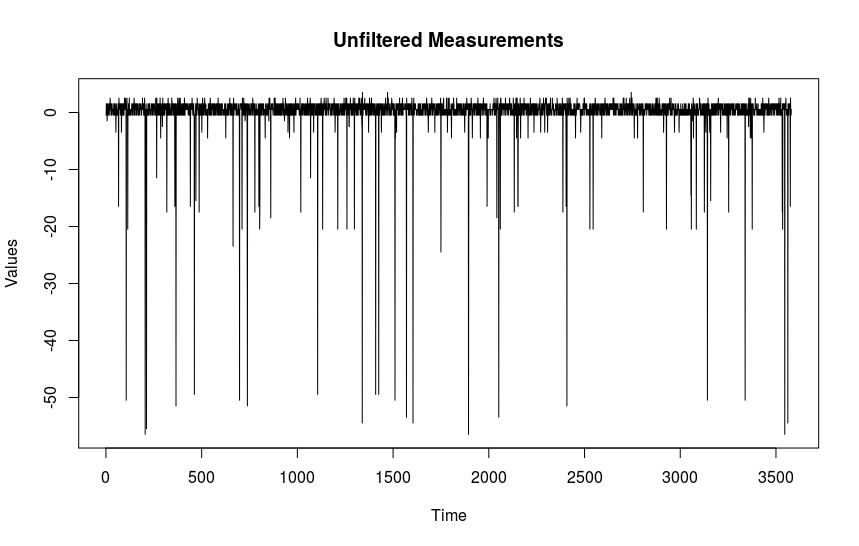
\includegraphics[width=.9\linewidth]{figures/UnfilteredZeroV1.png}
		\caption{RSSI values \cite{HORUS}}\label{fig:UnfilteredZero}
\end{figure}

And a summary of the values:
$$
\begin{array}{cccccc}
Min.& 1st Qu. & Median & Mean & 3rd Qu. & Max.\\
-87.00 & -31.00 & -30.00 & -30.53 & -29.00 & -27.00
\end{array}
$$
\section{Formal Description}
\subsection{First Filter}
The first one's mathematical model:
$y=(y_1,y_2\ldots y_n)$ is the filtered vector,$x=(x_1,x_2,\ldots x_n)$ is the starting value vector $ n\in \mathbb{N} $ is the number of values in the vector and $m \in \mathbb{N}$ is the memory size.
\begin{equation}\fontsize{15pt}{2}
y=(h(x,1,m),h(x,2,m)\ldots h(x,m,m), f(x,m+1,m)\ldots f(x,n,m))
\end{equation}
Where
\begin{equation}\fontsize{15pt}{2}
h(x,i,m)={(\sum\limits_{j=i}^{i+m-1}x_i) \over m}
\end{equation}
And
\begin{equation}\fontsize{15pt}{2}
f(x,i,m)=
\left\{
	\begin{array}{ccc}
	x_i & \mbox{if} |x_i-x_{i-1}|<t \\
	\\
	\overline{(x_i\ldots x_{i-m})} & \mbox{if} |x_i-x_{i-1}|>t
	\end{array}
\right.
\end{equation}           
The first part(h(x,i,m)):


The algorithm follows a simple pattern for the first 5 values. It takes the average from $x_i\ldots x_{i+m}$ indexes to create the filtered value of $y_1\ldots y_m$.
After the first m elements are calculated, it uses a different $f$ function to calculate the rest of the elements of y. 


The second  part(h(x,i,m)):

After the first 5 elements, the algorithm's actions are determined by a t variable.
If t is lesser than $|x_i-x_{i-1}|$, so the difference between the current and the last element exceeds the value of t:

the average of the last 5 $x$ value is put into the current y element.
If the previous condition is false, then the current x element is used as the filtered value.



\subsection{Second filter}
The second one's mathematical model:
$y=(y_1,y_2\ldots y_n)$ is the filtered vector,$x=(x_1,x_2,\ldots x_n)$ is the starting value vector $ n\in \mathbb{N} $ is the number of values in the vector and $m \in \mathbb{N}$ is the memory size.
The second filter's algorithm is much like the first one, except t is calculated after every iteration: 


\begin{equation}\fontsize{15pt}{2}
t=\sqrt{{1\over m}\sum\limits_{j=i}^{i-m}(x_j-\overline{x})^2}
\end{equation}



The second pard of the algorithm is different: 

The f function determines the elements by calculating a $t$ threshold that changes dynamically through the the function. It is always calculated by taking the standard deviation of the last 5 elements of the unfiltered vector. After the algorithm knows the value of t, it checks if the difference between the current element and the last element is greater than this value.

In the case that it is, it takes the average of the last m elements of the $X$ vector and puts it in the $y_i$ element.

If it's lesser then the t value, then $x_i$ is imply put into $y_i$.





\section{R Implementation} 
The implementations of the mathematical descriptions were done in R script.
The two filters are similar in nature, although offering different results.
The end results differ mildly depending on the choosing of threshold and memory size.
Choosing those two variables is key to an optimal filtering.
\subsection{First filter implementation}
The algorithm -- **
\begin{figure}[h!]
\fontsize{14}{2}
	\begin{lstlisting}
while(j<=memsize)
{
  i=1;
  while(i<=memsize)
  {
    a[i]<-Measurement$Signal[i+j-1]
    i=i+1
  }
  FilteredMeasurement$Signal[j]<-mean(a)
  j=j+1
}
	\end{lstlisting}
	\caption{The h(x,i,m) function, implemented.}\label{fig:code}
\end{figure}
\begin{figure}[h!]
\fontsize{14}{2}
	\begin{lstlisting}
while(x<=nrow(Measurement))
{
    if((abs(Measurement$Signal[x]-Measurement$Signal[x-1]))>thr)
    {
      i=1;
      while(i<=memsize)
      {
        a[i]<-Measurement$Signal[x-memsize+1+i]
        i=i+1
      }
      FilteredMeasurement$Signal[x]<-mean(a)
    }
    else
    {
      FilteredMeasurement$Signal[x]<-Measurement$Signal[x]
    }
  x=x+1
}
	\end{lstlisting}
	\caption{The f(x,i,m) function, implemented.}\label{fig:code}
\end{figure}

The following diagram and summary is after the filtering, with t and m chosen as 5:
\begin{figure}[h!]
	\centering
		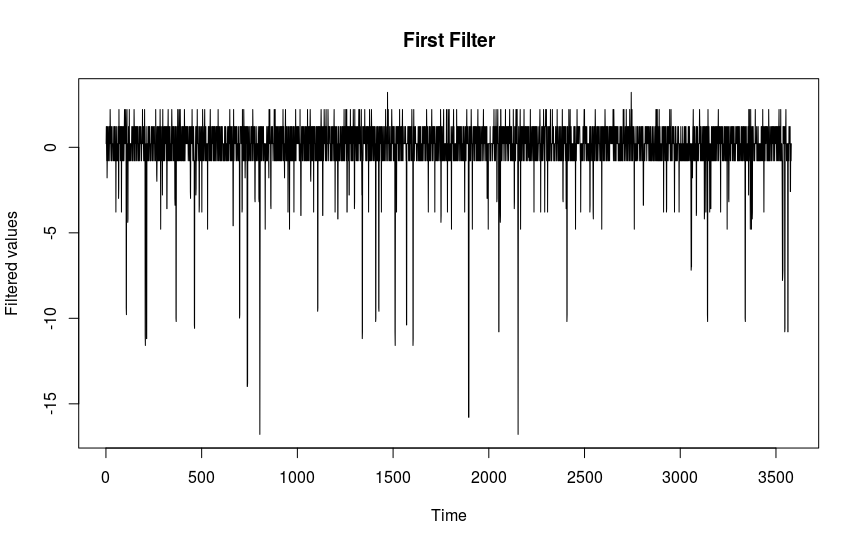
\includegraphics[width=.9\linewidth]{figures/FirstFilterZeroV1.png}
		\caption{Values with the first filter \cite{FirstFilter}}\label{fig:FirstZero}
		
		$$
		\begin{array}{cccccc}
		Min.& 1st Qu. & Median & Mean & 3rd Qu. & Max.\\
		-47.00 & -31.00 & -30.00 & -30.21 & -29.00 &   -27.00 
		\end{array}
		$$
		         
		
\end{figure}
\subsection{Second filter implementation}
Since the first part of the algorithm is analogous with the first one, it will not be included in this section.
The second part of the implementation is as follows:
\begin{figure}[h!]
\fontsize{14}{2}
	\begin{lstlisting}
while(x<=nrow(Measurement))
{
  thr<-(sd(a))*3
  i=1;
  while(i<=memsize)
  {
    a[i]<-Measurement$Signal[x - memsize + i]
    i=i+1
  }
  
  if((abs(Measurement$Signal[x]-Measurement$Signal[x - 1]))>thr)
  {
    FilteredMeasurement$Signal[x]<-mean(a)
  }
  else
  {
    FilteredMeasurement$Signal[x]<-Measurement$Signal[x]
  }
  x=x+1
}

	\end{lstlisting}
	\caption{The f(x,i,m) function, implemented.}\label{fig:code}
\end{figure} 


The following diagram and summary is after the filtering, with m chosen as 5:


\begin{figure}[h!]
	\centering
		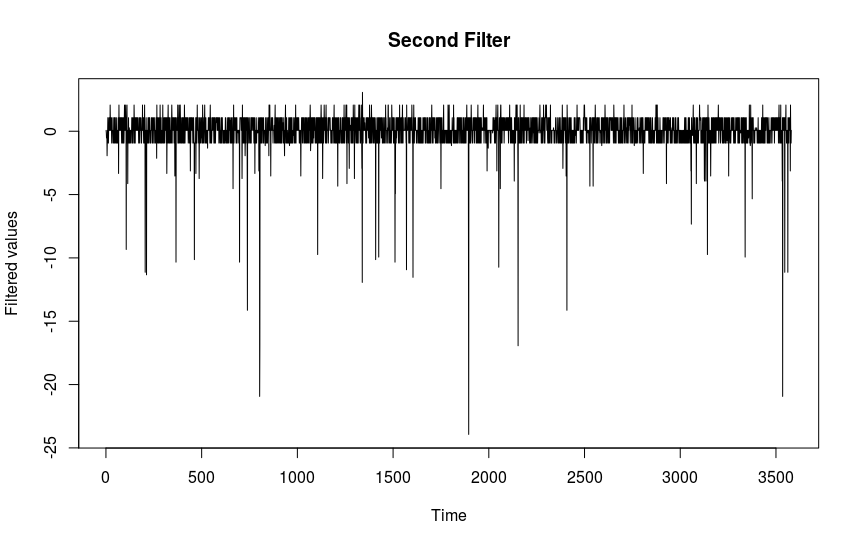
\includegraphics[width=.9\linewidth]{figures/SecondFilter.png}
		\caption{Values with the second filter \cite{secondzero}}\label{fig:SecondZero}
\end{figure}


\begin{figure*}
$$
		\begin{array}{cccccc}
		Min.& 1st Qu. & Median & Mean & 3rd Qu. & Max.\\
		-54.00 & -31.00 & -30.00 & -30.07  & -29.00 &-27.00 
		\end{array}
		$$
\end{figure*}
		          
		   